\documentclass[11pt]{article}

\usepackage{hyperref}
\usepackage{listings}
\usepackage{color}
\usepackage{xcolor}
\usepackage{caption}
\usepackage[T1]{fontenc}
\usepackage{lmodern}
\usepackage{graphicx}
\usepackage{comment}
\usepackage{underscore}


%\DeclareCaptionFont{white}{\color{white}}
%\DeclareCaptionFormat{listing}{\colorbox{gray}{\parbox{\textwidth}{#1#2#3}}}
%\captionsetup[lstlisting]{format=listing,labelfont=white,textfont=white}

\DeclareCaptionFont{white}{\color{white}}
\DeclareCaptionFormat{listing}{\colorbox[cmyk]{0.43, 0.35, 0.35,0.01}{\parbox{\textwidth}{\hspace{15pt}#1#2#3}}}
\captionsetup[lstlisting]{format=listing,labelfont=white,textfont=white, singlelinecheck=false, margin=0pt, font={bf,footnotesize}}

\lstset{ %
language=[Objective]C, 
%breakindent=40pt,
basicstyle=\ttfamily\footnotesize,       % the size of the fonts that are used for the code
%numbers=left,                   % where to put the line-numbers
numberstyle=\ttfamily\footnotesize,      % the size of the fonts that are used for the line-numbers
%stepnumber=1,                   % the step between two line-numbers. If it is 1 each line will be numbered
numbersep=5pt,                  % how far the line-numbers are from the code
backgroundcolor=\color{white},  % choose the background color. You must add \usepackage{color}
showspaces=false,               % show spaces adding particular underscores
showstringspaces=false,         % underline spaces within strings
showtabs=false,                 % show tabs within strings adding particular underscores
%frame=single,           % adds a frame around the code
%frame=shadowbox,
%frame=tb,
tabsize=2,          % sets default tabsize to 2 spaces
%captionpos=b,           % sets the caption-position to bottom
breaklines=true,        % sets automatic line breaking
breakatwhitespace=false,    % sets if automatic breaks should only happen at whitespace
escapeinside={\%*}{*)},          % if you want to add a comment within your code
%stringstyle=\color{white}\ttfamily,
 xleftmargin=17pt,
         framexleftmargin=17pt,
         framexrightmargin=5pt,
         framexbottommargin=4pt
}

\author{Victor Lazzarini, Steven Yi and Martin O'Shea}
%\date{2012.08.xx}
\date{\today}
\title{Csound for Android}

\begin{document}
\maketitle

\section{Introduction}

Welcome to Csound for Android! This document will discuss the details about using Csound for Android OS using the Eclipse IDE.  

For those with knowledge of Csound, hopefully you will see that the value of your knowledge is only enhanced by offering a new platform on which to create musical software and works. 

\subsection{Regarding the Csound for Android Examples Project}

This documentation covers discussion of the Csound for Android API.  Users interested in diving in to see how the API is used may want to download the Csound for Android Examples Project which contains a set of examples that cover different use cases of the API. The code for each example may be useful in giving you a jump-start in building your own application.

\subsection{Regarding the LGPL License}

The Csound for Android includes Csound and \href{http://mega-nerd.com/libsndfile/}{libsndfile}. These are distributed as static libraries. Users of the Csound for Android API must comply with the licensing requirements of the GNU Lesser General Public License v2.1, which both libraries use. Please carefully review the license files that accompany each project (you can view a generic version of the LGPL v2.1 license at \href{http://www.gnu.org/licenses/lgpl-2.1.html}{http://www.gnu.org/licenses/lgpl-2.1.html}). 

%======

\section{Getting and Using the Csound for Android API}

The Csound for Android library is distributed as a Zip release from the Csound Sourceforge page. The Zip archive includes:

\begin{itemize}
\item Statically compiled libcsound.a and libsndfile.a, compiled as universal binaries for armv6, armv7, and i386 CPU architectures (to work with both Android devices and simulators)
\item C Headers for the Csound C API
\item Java API source
\item Documentation
\end{itemize} 

You will also need to install the android NDK available at \href{http://developer.android.com}{AndroidDeveloper} site, to compile the native code in Csound for java.

Csound for Android was chosen to be delivered as pre-compiled libraries and headers for easy inclusion into projects.  After starting a new project in Eclipse, do the following:

\begin{enumerate}
\item Import the CsoundAndroid Library into Eclipse using file>import from the location you downloaded it to.
\item Right-click your project and from the context menu choose ``Properties''
\item In the window that opens, select the "Android tab" on the left hand-side of the window,  go to the right of the box labelled "library" select "add". Select the "CsoundAndroid Library" which you have just added to your workspace(Step 1).
\item If at anytime when working with the CsoundAndroid library the project does seem not to recognise the CsoundAndroid is added, select "Project" from the menu bar and then select "Clean" to rebuild the paths in the project. 
\end{enumerate}

After adding the CsoundAndroid library, it should now be a part of your project. You will now be able to reference both the standard Csound C API as well as the Java CsoundObj API from your project code.

%======

\section{Introduction to the API}
\subsection{CsoundObj and Csound API's}

Csound for Android is released with the standard Csound C API as well as a custom Java CsoundObj API that has been designed to make developing on Android OS convenient.  The CsoundObj API includes methods for binding widgets to channels (used to communicate to and from Csound), enabling hardware sensors, and more.  For further detail, please consult the CsoundObj.java class.

While the CsoundObj API has been designed to ease things for Android OS development and to follow conventions of Java, the decision was made not to wrap everything in the Csound C API. . The Csound java Object that a CsoundObj class holds can be accessed via the \textbf{getCsound} method in CsoundObj.  For more information about the Csound C API, consult Csound.java class.

\section{Using the CsoundObj API}

The CsoundObj API revolves around the Java CsoundObj class. This class contains a Csound Object and has methods for running Csound, as well as convenience methods to help aid developers in connecting elements to Csound. By itself, CsoundObj can take in a CSD file and render it.  By using CsoundBindings, objects can interact to read values from and write values to Csound.  Beyond that, extended features can be accessed by using the Csound C API together with the Csound object.

\subsection{Designing Csound CSD projects to work with Hosts}

To communicate to and from a host program with Csound, you will most likely use \textbf{chnset} and \textbf{chnget} opcodes. These opcodes will allow you to read from and write values to a named channel.  Your host program will also be writing to and reading from these same channels.  As a byproduct of using named channels, your CSD will be portable to work on other platforms (Desktop, IOS); porting over apps to/from Android then will only involve redoing the application and UI code, while your audio engine (Csound) should ``just work.'' 

\subsubsection{CsOptions}

Csound will use the CsOptions you provide.  A standard set of flags to use are ``{\tt -odac -dm0 -+msg\_color=0}''. This will tell Csound to play to dac in realtime, turn off displays, use message level 0, and turn of message colors.  This will minimize messages going out to the console or to your message handler if you set one.  You may also need ``{\tt -iadc}'' if your project uses audio input. (You can always consult the Csound Examples project to see what CsOptions are used in the CSD's for that project.) 

\emph{Note: In Csound5 for Android, it was previously required to set \linebreak ``{\tt -+rtaudio=null}'' when using audio. This is no longer required for Csound 6 for Android.}
 

\subsection{CsoundBinding for Communicating with Csound}

The CsoundObj API has been created to ease communication with Csound by using objects that implement the CsoundBinding interface.  The interface definition is as follows:

\begin{lstlisting}[caption=CsoundBinding interface Definition]

public void setup(CsoundObj csoundObj);
	
public void updateValuesToCsound();
	
public void updateValuesFromCsound();
	
public void cleanup();

\end{lstlisting}

CsoundBindings are used to both read values from Csound as well as write values to Csound.  The lifecycle of CsoundBindings is as follows:

\begin{itemize}
\item \textbf{setup} - this has now been changed. This method is called after Csound's compile call but before the main performance loop. CsoundBindings should use this method to cache any channel pointers and any other values they will need during performance.
\item \textbf{updateValuesToCsound} and \textbf{updateValuesFromCsound} - these methods are called during the Csound performance loop. \textbf{updateValuesToCsound} is called before each call to csoundPerformKsmps, while \textbf{updateValuesFromCsound} is called after each call. 
\item \textbf{cleanup} - this method is called after Csound has completed its run and should be used by CsoundBindings to free up any allocated data and remove references to channel pointers.
\end{itemize}

By using CsoundBindings, CsoundObj functionality can be extended to communicate with as many items as you would like. The Csound for the Android API contains pre-made wrapper classes for common UI classes (Slider, Button) as well as hardware sensors (Accelerometer).  CsoundObj has helper methods for the CsoundBindings that come with the CsoundObj API, as well as the generic \textbf{addBinding} and \textbf{removeBinding} methods for adding custom CsoundBindings. Please consult these classes as well as their use in context within the Csound for Android Examples project.


%======

\section{Common CsoundObj API Methods}

\subsection{Binding Widgets to CsoundObj}

The CsoundObj API contains the following methods for binding widgets:

\begin{lstlisting}[caption=Methods for Widget Binding]
public CsoundBinding addButton(Button button, String channelName))
public CsoundBinding addButton(Button button, String channelName,int type)
public CsoundBinding addSlider(SeekBar seekBar, String channelName, double min, double max)}

These methods allow for easy binding of UISeekBars, and UIButtons, and return the CsoundBinding that was created to wrap the widget. If the design of your app requires that you remove a widget from being used with CsoundObj, you can use the returned CsoundBinding and pass it to the removeCsoundBinding method. To bind your own custom widgets, you will need to create your own CsoundBinding.  There are examples of both using the convenience widget binding methods as well as custom CsoundBindings in the Csound for Android Examples project.
\end{lstlisting}
%======

\section{Interfacing with Hardware}
\subsection{Audio Input and Output}

CsoundObj has been designed to connect everything necessary for audio input and output from Csound to \textit(OpenSL) in the when the CsoundLib Library is compiled in with the NDK, the CsoundObj can also interact with audio track at run time (this is to allows for  downward compatibility with 2.2 and lower).  Enabling input and output depends on what commandline arguments are given when running Csound.  The commandline arguments should be supplied as part of the CSD's \textbf{CsOptions} section.  To enable audio output, use \textbf{-o dac} and to enable audio input, use \textbf{-i adc}. 

\subsection{Accelerometer}

CsoundObj has built-in support for use of the accelerometer found in android devices. CsoundObj has the following methods to enable these features:


\begin{lstlisting}[caption=CsoundObj Accelerometer Method]
public CsoundBinding enableAccelerometer(Context context)
]
\end{lstlisting}

When the feature is enabled, CsoundBindings that wrap the sensor will send values into Csound via hardcoded channels:

\begin{itemize}

\item Acclerometer
\begin{itemize}
\item accelerometerX
\item accelerometerY
\item accelerometerZ
\end{itemize}

\end{itemize} 

Once a sensor has been enabled, you can access those values in Csound using \textbf{chnget}. For further study, please see the \emph{Hardware Test} example in the Examples project. 

%======

\section{Csound for Android Examples}

The Examples project contains a number of simple examples that illustrate different aspects of working with Csound for Android.  The following is a brief description of each of the examples.

\subsection{Simple Test 1}

Simple example that plays ascending notes.  The pitch of the notes can be altered by using the SeekBar.  Also, a ToggleButton is used to turn on/off the rendering of Csound.  In the code, you'll find that the callback that is connected to the ToggleButton shows the basic usage of CsoundObj to render a CSD that is included as a resource for the project:

\begin{lstlisting}[caption=Example code showing configuring and starting a CsoundObj]
public void onCheckedChanged(CompoundButton buttonView, boolean isChecked) {
				if(isChecked) {
					String csd = getResourceFileAsString(R.raw.test);
					File f = createTempFile(csd);
					csoundObj.addSlider(fSlider, "slider", 0.,
							1.);
					csoundObj.addListener(SimpleTest1Activity.this);
					csoundObj.startCsound(f);
				} else {
					csoundObj.stopCsound();
				}
				
			}
		});
\end{lstlisting}

\subsection{Simple Test 2}

This is a generative music example that contains a number of SeekBars that affect the rate of notes generated, the duration of notes, and the ADSR envelope for each note. 


\subsection{Button Test}

This example uses a CSD based on the one used for Simple Test 2, but depends on the user to trigger a button to generate each note.  The two buttons in this example show two different ways in which to integrate buttons with CsoundObj:

\begin{enumerate}
\item Using CsoundObj's \textbf{addButton} method, which will setup a k-rate channel for Csound, the value will be 0 when the button is not pressed, and will be 1 for one ksmps period when a button is pressed (it returns to 0 the following ksmps period). 
\item Using a standard button callback, the callback will create a string score and send that to Csound using CsoundObj's \textbf{sendScore} method. (See code below.)
\end{enumerate}


\begin{lstlisting}[caption=Example code showing sending score text to CsoundObj]
String event = String.format("i2 0 %f", value);
									
csoundObj.sendScore(event);
\end{lstlisting}

Note that the second method will read the value from the duration slider when creating the note, while the first method handles reading the duration from the channel within the CSD code. 

\subsection{Ping Pong Delay}

This example shows processing audio input in realtime, using a Ping Pong Delay. The use of audio input is controlled by the standard Csound flag \textbf{-i adc} that is found in the CSD's \textbf{CsOptions} section.  


\subsection{Harmonizer}

This example highlights the same techniques as the Ping Pong Delay, but shows the use of Csound's streaming Phase Vocoder to create a harmonizer effect. 

\subsection{Accelerometer}

This example shows the use of the accelerometer sensor.  For this example, the accelerometer is enabled and values are read by the CSD to affect the pitch of a vco2 oscillator, as well as cutoff and resonance of a moogladder filter. 

\subsection{Csound Haiku 4}

\emph{Csound Haiku} is a generative art music work by Iain McCurdy.  Number 4 from this set of pieces was chosen to exercise what this platform is of capable.

\subsection{Multitouch XY}

This example demonstrates a multitouch performance surface. The multi-touch code maps each touch down and up to a note on and off.  It also sends continous x and y values to Csound.  The Csound programming in the CSD shows a technique for doing individual per-note control data mapping by dynamically assigning what channels of data each note should read from. 

\subsection{Waveview}

This example demonstrates using a CsoundBinding to read an f-table from Csound and displaying that table.  Note that the WaveView's code is doing some optimization to check if it has already loaded.  It is also checking that the table itself has completed loading before trying to grab any values for the table. 

\begin{lstlisting}[caption=Waveview code demonstrating reading f-tables from Csound]
		public void updateValuesFromCsound() {
			if (!tableLoaded) {
				Csound csound = csoundObj.getCsound();
				CsoundMYFLTArray table = new CsoundMYFLTArray();
				int length = csound.TableLength(1);
				csound.GetTable(table.GetPtr(), 1);
				tableData = new double[length];

				for (int i = 0; i < length; i++) {
					tableData[i] = table.GetValue(i);
				}

				tableLoaded = true;

				new Thread() {
					@Override
					public void run() {

						int width = getWidth();
						int height = getHeight();
						int middle = height / 2;

						points = new int[width];

						int tableLength = tableData.length;

						for (int i = 0; i < width; i++) {
							float percent = i / (float) (width);
							int index = (int) (percent * tableLength);
							points[i] = (int) ((tableData[index] * middle) + middle);
						}

						postInvalidate();

					}
				}.start();
			}
		}
\end{lstlisting}



%======
\section{Making Your First Csound Android App }
This section will walk you through your first implementation of the Csound library for Android: 
\begin{itemize}
\item assuming you have added the library to your project as explained in the \textit{Getting and Using the Csound for Android API} section; and
\item  that your application is called \textit{First_Csound_App} with the package name of \textit{com.example.first_csound_app}; and
\item you used the default names for your first class and xml file, which are\textit{MainActivity.java}  and  \textit{activity_main.xml}  respectively
\end{itemize}

 First let us create the user interface. This is simplest using xml files, though this can be achieved through Java.

First navigate to the $res>layout>$\textit{activity_main.xml} in the Package explorer in Eclipse. At the bottom left of the the xml view pane you will see a graphical layout tab and an activity_main.xml tab
\begin{center}

\includegraphics{images/xmlTabBar}
\end{center}

Insert the following code in the xml file. This will create three Buttons and a SeekBar as shown.
\begin{lstlisting}[caption=Code to create UI]
<RelativeLayout xmlns:android="http://schemas.android.com/apk/res/android"
    xmlns:tools="http://schemas.android.com/tools"
    android:layout_width="match_parent"
    android:layout_height="match_parent" >
    
    <!--This is a comment! the following inserts a Button and is 
    soley responsiple for how the Button looks in this app.
    The id section is used for refferencing to the Button throughout
    the rest of the project -->
    
    <LinearLayout 
        xmlns:android="http://schemas.android.com/apk/res/android"
        android:id="@+id/ButtonList"
        android:orientation="horizontal"
        android:layout_width="match_parent"
        android:layout_height="wrap_content"
        >
    <Button
        android:id="@+id/StartCsound"
        android:layout_width="wrap_content"
        android:layout_height="wrap_content"
        android:layout_centerHorizontal="true"
        android:text="StartCsound"
         />
    <Button
        android:id="@+id/StopCsound"
        android:layout_width="wrap_content"
        android:layout_height="wrap_content"
        android:layout_centerHorizontal="true"
        android:text="StopCsound"
         />
    <Button
        android:id="@+id/Button1"
        android:layout_width="wrap_content"
        android:layout_height="wrap_content"
        android:layout_centerHorizontal="true"
        android:text="B1"
         />
    
    </LinearLayout>
    
    <!--This is a comment! the following inserts a SeekBar (comminly reffered to as a slider) and is 
    soley responsiple for how the Button looks in this app.
    The id section is used for refferencing to the SeekBar throughout
    the rest of the project-->
    <SeekBar
        android:id="@+id/SeekBar1" 
        android:layout_width="fill_parent"
        android:layout_height="wrap_content"
        android:layout_centerHorizontal="true"
        android:layout_below="@+id/ButtonList"
        />

</RelativeLayout>
\end{lstlisting}

\begin{center}
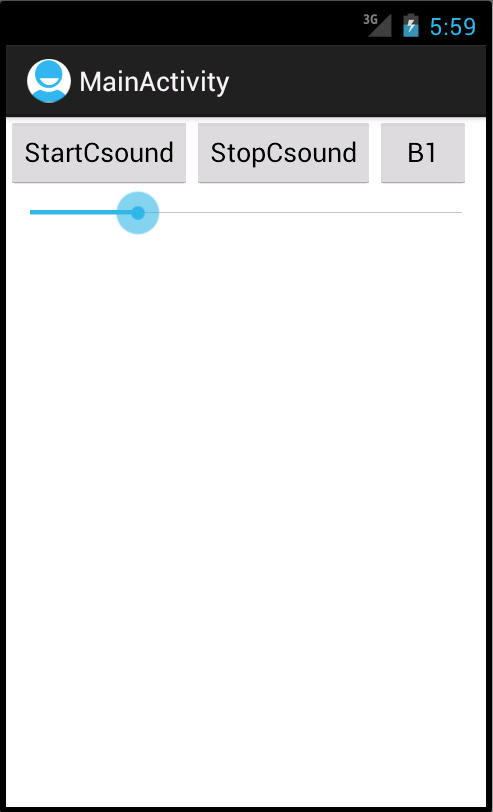
\includegraphics[scale=0.30]{images/CsoundBasicAppUIDia}
\end{center}

Next go to your project manifest to add the necessary permissions for fully using the CsoundObj. This is done by selecting AndroidManifest.xml from the package explorer, then selecting  \textit{AndroidManifest.xml} from tabs at the bottom of the main pane

\begin{center}

\includegraphics[scale=0.75]{images/ManifestTabs}
\end{center}

Adding the following to your Manifest

\begin{center}
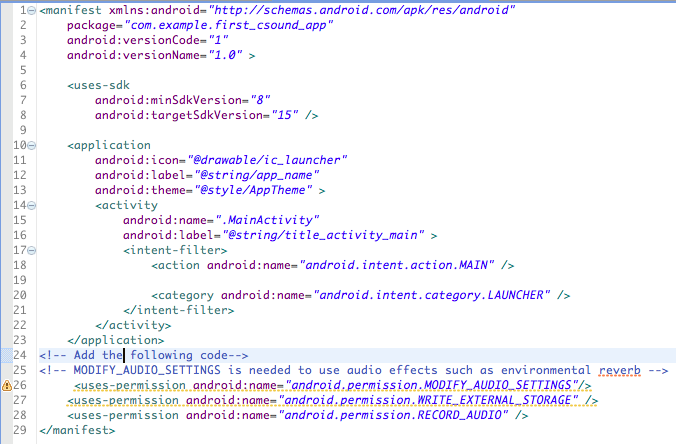
\includegraphics[scale=0.60]{images/Manifest}
\end{center}

Now that the UI is built and the manifest has been prepared, proceed to opening the main activity of the project \textit{src}$>$\textit{com.example.first_csound_app}$>$\textit{MainActivity.java}. You should see the following when you open the class (depending on your Eclipse preferences the line numbering may not appear)
\begin{center}
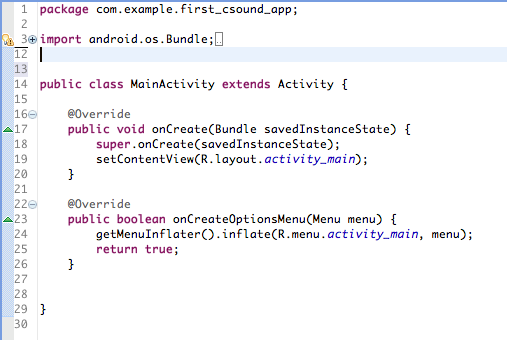
\includegraphics[scale=0.75]{images/CsoundBasicAppOrignalActivity}
\end{center}

First add the \textit{BaseCsoundActivity.java} class to your project. This can be done by copying it into the \textit{src} folder of your project on your computer from the CsoundAndroidExamples project that comes with the Csound for Android download.

Next you need to import the necessary packages into your package for the application to compile correctly. These include the Csound package and widget packages for the UI. To see all the automatically imported packages click the $+$ button beside the import shown in the last image

\begin{center}
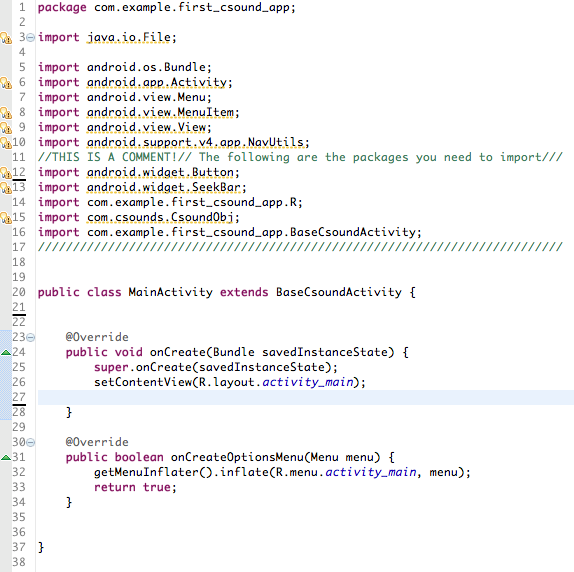
\includegraphics[scale=0.60]{images/ImportedPackages}
\end{center}


Next extend your class with BaseCsoundActivity instead of Activity (note that BaseCsoundActivity extends Activity). Then  add your variables and then initialise them in the onCreate method as shown below. 

\begin{center}
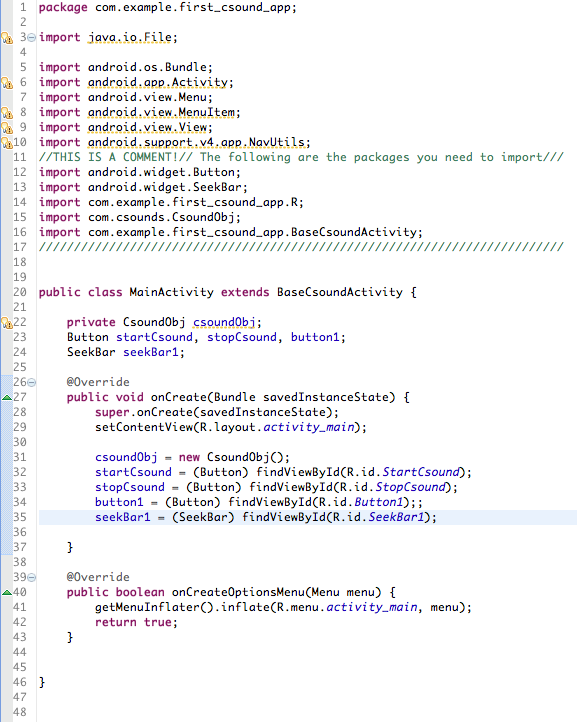
\includegraphics[scale=0.60]{images/VariblesCreated}
\end{center}

Finally in our Activity class we have to connect our UI comments to our CsoundObj to allow us to pass information from our UI to our Csound code. In following code the max value of the SeekBar is set to 1 and the minium value is set to 0. To reserve this data in your Csound code use the opcode chnget and button1 and seekBar1. The button and SeekBar are added each time before every time CsoundObj is set playing to ensure they are in the variable cacheable for the object

\begin{center}
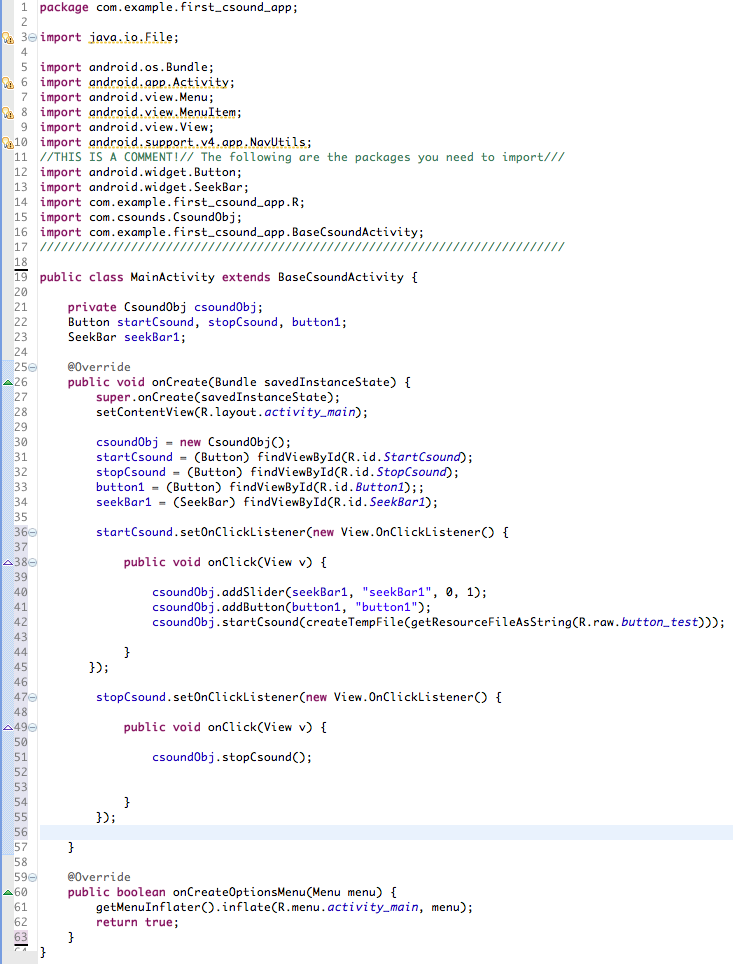
\includegraphics[scale=0.50]{images/FinalActivity}
\end{center}

Finally, to get your Csound code into the project, create a \textit{raw} folder in your project in the \textit{res} folder. This can be done by right clicking your  \textit{res} folder in your package explorer in Eclipse, from the drop down menu set \textit{new} followed by \textit{folder} then name the folder  \textit{raw}. 

\begin{center}
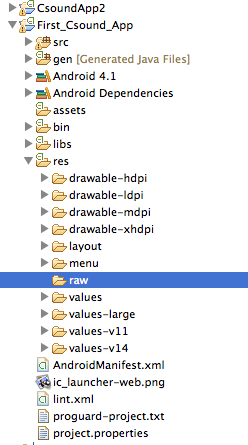
\includegraphics[scale=0.60]{images/PackageExplorer}
\end{center}

Next go to the containing folder of your project on your computer and put your Csound .csd file in the raw folder. Now when you return to Eclipse and run your project as an \textit{Android Application} by clicking the play button in Eclipse, Your first Csound app should be running with your Csound code, congratulations!


\section{Csound App 2.0}
This app demonstrates the use of the Csound library in the context of a larger application with multiple Activities, Views and the ability to load in different .csd files dynamically. It is designed for stand alone use for those that do not want to get their hands dirty with Android programming but still want access to the platform, and for those who want an app with lots of functionality that they can use in their own applications. 

Hence the in order to get up and running with Csound on Android, all you need to do is use chnget in your .csd to get access to the UI values. SeekBars are set from 0 to 1 consequently some scaling may be necessary in your .csd. The Variable names to be used are:

\begin{itemize}
\item Performance1
\begin{itemize}
\item seekBar1
\end{itemize}
Performance 2
\begin{itemize}
\item seekBar2
\end{itemize}
Mixer
\begin{itemize}
\item seekBar3
\item seekBar4
\item seekBar5
\item seekBar6
\item seekBar7
\item seekBar8
\end{itemize}
\end{itemize}

\begin{itemize}
\item Performance1
\begin{itemize}
\item B1
\item B2
\item B3
\item B4
\item B5
\item B6
\item B7
\item B8
\item B9
\item B10
\item B11
\item B12
\item B13
\item B14
\item B15
\item B16
\item B17
\item B18
\item B19
\end{itemize}
Performance 2
\begin{itemize}
\item B20
\item B21
\item B22
\item B23
\item B24
\end{itemize}
\end{itemize}

\begin{lstlisting}[caption=Exampe of code to be used in .csd to connect Seekbars and Buttons]
kVolume chnget "seekBar1"
kOnOff  chnget "B1"
\end{lstlisting}

To use the xy pad in tab Performance2 use the following
\begin{lstlisting}[caption=Exampe of code to be used in .csd to connect xy pad]
S_xName sprintf "touch.%d.x", i_instanceNum
S_yName sprintf "touch.%d.y", i_instanceNum

kx chnget S_xName
ky chnget S_yName
\end{lstlisting}

For those who want to customise the app and understand its workings the following, along with the comments in the apps code should help. This application has been designed to allow user changes to the source code and was built to demonstrate the use of a singleton design process to preserve a CsoundObj for the whole Android lifecycle of an application. There are several situations that have to be taken into consideration.

\begin{enumerate}
\item Adding the UI controls to the CsoundObj when Android Activities are created and destroyed by the Android OS to recover RAM.
\item The selecting of new .csd files to be loaded into the application, and creating a new CsoundObj object for this event. 
\item The consistency between different activities and views to allow users to change between views during a performance.
\end{enumerate}

Many of these features are achieved by extending Application. It is used to store the CsoundObj, the current file path, the current features of each application and view. it is also used to give all activities a set of methods which will always have to be called and which will never be destroyed by the Android life cycle, thus ensuring their constant availability
It is important to note that throughout this app BaseCsoundActivity.java is extended instead of Activity (As BaseCsoundActivity.java extends Acitivity). BaseCsoundActivity.java is used to take advantage of it methods such as:
\begin{itemize}
\item protected String getResourceFileAsString(int resId)
\item protected File createTempFile(String csd)
\end{itemize}
Hence this may be a design choice worth remembering when coding your own apps.

\section{Conclusion}

We hope that this document has helped you to become familiar with the design and usage of the Csound for Android API. The example Java and Csound CSD code should hopefully give you a good starting point for your own musical projects, and we encourage you to take these examples and run with it.  We look forward to hearing your questions and feedback on this API, and most of all, look forward to seeing what you will create with all of this.  Best of luck and enjoy! 

\end{document}
